\documentclass[12pt, letterpaper]{report}
\usepackage{graphicx}
\usepackage{hyperref}
\usepackage{amssymb}
\usepackage{amsmath}
\usepackage{float}
\usepackage{mathtools}
\usepackage{enumitem}
\usepackage[margin=1in]{geometry}
\usepackage[figurename=Figura]{caption}
\title{Examen Argumentativo 1, Módulo Física}
\author{Juan Pablo Guerrero Escudero, A01706810}
\date{27 abril, 2024}
\begin{document}
\maketitle
\subsection*{Selfie}
\begin{figure}[H]
    \centering
    
\includegraphics[height = 5cm]{Selfie.jpeg}
    \caption{Selfie después de terminar mi examen argumentativo}
\end{figure}
\subsection*{Situación 1}
Un Inge con mucho tiempo libre (gracias a su desafortunada vida amorosa), realiza un experimento mental. Decide crear un escenario electrostático para demostrar sus habilidades teóricas y computacionales. Coloca una carga puntual en cada esquina de un cuadrado de lado a. Cada carga tiene una magnitud q, donde dos son positivas y dos son negativas, dispuestas alternadamente (ver figura). Como buen Inge, quiere calcular la intensidad y la dirección de la fuerza resultante en el centro del cuadrado para asegurarse de que su demostración no será un desastre apocalíptico.

Pregunta teórica: Determina la intensidad de la fuerza y su dirección en el centro del cuadrado en términos de q y a (una fórmula). Asume que el espacio es el vacío y utiliza la Ley de Coulomb para tu análisis.

Pregunta práctica: Suponiendo que q es igual a la magnitud de la carga de un electrón y a es igual a 0.20 nm. Utiliza tu simulador de Coulomb (MATLAB) para verificar tu cálculo anterior. Documenta cualquier diferencia o confirmación.

Recuerda: Aunque en el amor y en la electrostática las atracciones son importantes, ¡asegúrate de que tus respuestas sean argumentativas! \\

\textbf{Solución: } En primer lugar, debido a que trabajamos con cargas eléctricas en la situación dada, es conveniente usar la Ley de Coulomb para analizar la fuerza eléctrica, ya que 
trabajamos con cargas puntuales, y lo que la ley de Coulomb nos permite hacer es calcular la Fuerza eléctrica ejercida sobre una carga específica por otras cargas puntuales en el sistema. 
En segundo lugar, debido a que tenemos cuatro cargas acomodadas de manera simétrica, y queremos saber la fuerza eléctrica en el centro del cuadrado del lado $a$, donde en cada esquina se encuentra 
una carga puntual, es conveniente establecer un sistema de coordenadas cartesianas, seleccionando el centro del cuadrado como el origen, es decir, el punto $(0, 0)$.\\ 

Después, conviene usar el principio de superposición, que establece que la fuerza resultante ejercida sobre una carga es igual a la suma de las fuerzas individuales 
que cada una de las otras cargas ejerce sobre ésta. Es decir, $\vec{F}_{neta} = F_{21} + F_{31} + ... + F_{n1}$. 
Entonces, podemos calcular la fuerza eléctrica neta sobre el centro de la carga usando la suma de fuerzas, calculadas con la Ley de Coulomb, y obtener una fórmula para ésta: \\

Para ésto, definimos las posiciones de las cuatro cargas, $q_1 = (-\frac{1}{2}a, \frac{1}{2}a)$, $q_2 = (\frac{1}{2}a, \frac{1}{2}a)$, siendo ambas cargas positivas con magnitud $+q$ que se encuentran 
en las esquinas superiores del cuadrado, y 
$q_3 = (-\frac{1}{2}a, -\frac{1}{2}a)$, $q_4 = (\frac{1}{2}a, -\frac{1}{2}a)$, con magnitudes $q_3 = q_4 = -q$, que son las cargas en las esquinas inferiores del cuadrado. Por último, definimos la carga en el centro $q_0$ con posición $(0, 0)$.\\ 

Ahora, como la Ley de Coulomb nos ofrece magnitud y dirección usando su fórmula $F_e = \frac{kq_0 q_1}{R^3}\vec{R}$, necesitamos calcular los vectores de separación $R_n$ entre cada una de las cargas y la carga $q_0$. Éstos se calculan con una resta de 
vectores, restando el punto final menos el punto inicial. Entonces, ahora se calculan éstos: 
\begin{align}
R_1 &= (0, 0) - (-\frac{1}{2}a, \frac{1}{2}a) = (\frac{1}{2}a, -\frac{1}{2}a)\\
R_2 &= (0, 0) - (\frac{1}{2}a, \frac{1}{2}a) = (-\frac{1}{2}a, -\frac{1}{2}a) \\ 
R_3 &= (0, 0) -  (-\frac{1}{2}a, -\frac{1}{2}a) = (\frac{1}{2}a, \frac{1}{2}a)\\
R_4 = &= (0, 0) -  (\frac{1}{2}a, -\frac{1}{2}a) = (-\frac{1}{2}a, \frac{1}{2}a)
\end{align}
Ahora, podemos calcular la magnitud de cada vector de separación, pero nos damos cuenta que como el sistema es simétrico, tienen la misma magnitud, es decir, $|R_1| = |R_2| = |R_3| = |R_4|$. Y solo basta con calcular uno de ellos. Calculamos entonces $|R_1|$: 
\begin{align}
|R_1| &= \sqrt{(\frac{1}{2}a)^2 + (-\frac{1}{2}a)^2} = \frac{\sqrt{x^2}}{\sqrt{2}} = \frac{a}{\sqrt{2}}
\end{align}
Ahora, ya que tenemos las posiciones y magnitudes de las cargas en el sistema, y los vectores de separación y sus magnitudes, 
usando el principio de superposición podemos calcular la fuerza total sobre la carga $q_0$ en el centro del cuadrado: 
\begin{align}
\vec{F}_{neta} &= \vec{F}_{15} + \vec{F}_{25} + \vec{F}_35 + \vec{F}_45\
\end{align}
Usando la Ley de Coulomb para cada fuerza individual, donde $k$ representa la constante de Coulomb, con valor de $9x10^9 C$:
\begin{align}
\vec{F}_{neta} &= \frac{kq_1q_0}{(\frac{a}{\sqrt{2}})^3}(R_1) + \frac{kq_2q_0}{(\frac{a}{\sqrt{2}})^3}(R_2) + \frac{kq_3q_0}{(\frac{a}{\sqrt{2}})^3}(R_3)
+ \frac{kq_4q_0}{(\frac{a}{\sqrt{2}})^3}(R_4)
\end{align}
Podemos reescribir el denominador de cada fuerza individual como $\frac{a^3}{2\sqrt{2}}$ gracias a las leyes de los exponentes, y al reescribir la fórmula anterior podemos utilizar la recíproca del denominador, y así 
pasamos $2\sqrt{2}$ hacia el numerador: 
\begin{align}
\vec{F}_{neta} &= \frac{kq_1q_0 2\sqrt{2}}{a^3}(R_1) + \frac{kq_2q_0 2\sqrt{2}}{a^3}(R_2) + \frac{kq_3q_0 2\sqrt{2}}{a^3}(R_3) + \frac{kq_4q_0 2\sqrt{2}}{a^3}(R_4)
\end{align}
Ahora, podemos factorizar el resultado anterior para simplificar más la fórmula de la fuerza neta:
\begin{align}
\vec{F}_{neta} = \frac{kq_02\sqrt{2}}{a^3}(q_1 \vec{R}_1 + q_2 \vec{R}_2 + q_3 \vec{R}_3 + q_4 \vec{R}_4)
\end{align}
Y así, como cada vector separación es un vector, y como de acuerdo al problema podemos decir que $q_1 = q_2 = q$, y $q_3 = q_4 = -q$, podemos ver que lo que resulta es que se está escalando cada vector por la magnitud de su carga correspondiente, por lo que al hacer 
el producto de cada escalar de carga $q_n$ por su vector de separación $R_n$, y luego hacer la suma de vectores, obtenemos el siguiente resultado: 
\begin{align}
\vec{F}_neta = \frac{kq_02\sqrt{2}}{a^3}(0, -2aq)
\end{align}Ésto lo que nos dice es que la fuerza resultante solo tiene componente en $y$, y está direccionada hacia abajo, o el eje $y$ negativo. Si multiplicamos éste último vector resultante por todo el valor constante $\frac{kq_02\sqrt{2}}{a^3}$, obtenemos 
la fórmula final: 
\begin{align}
    \vec{F}_{neta} &= \frac{kq_02\sqrt{2}}{a^3}(0)\hat{x} - \frac{2aqkq_02\sqrt{2}}{a^3}\hat{y}\\
    \vec{F}_{neta} &= -4(\frac{kqq_0\sqrt{2}}{a^2})\hat{y}
    \label{eq:eq1}
\end{align}Y así, la fórmula \ref{eq:eq1} representa una fórmula para obtener la magnitud y dirección (la cuál solo tiene componente en $y$) de la 
fuerza eléctrica neta aplicada por las cuatro cargas en las esquinas del cuadrado. Ésto es congruente ya que como estamos trabajando en un sistema eléctrico y con simetría, 
esperamos que la fuerza resultante termine en una sola dirección, que en éste caso al ser la carga de prueba $q_0$ positiva, se ve atraida hacia las cargas inferiores que son negativas, 
y se repele de las cargas superiores que son positivas, y por lo tanto la dirección de la fuerza resultante termina siendo en $y$ negativa. \\

Ahora, continuando con la parte práctica, si suponemos que $q = 1.6x10^-19 C$, y que $a = 2x10^-10m$, la fórmula anterior resulta $\vec{F}_{neta} = 
-2.0365x10^{11}q_0 \hat{y} N$. Ésto lo podemos comprobar con Matlab, con el simulador hecho previamente en el curso, que, ingresadas las magnitudes 
y posiciones de un sistema de cargas, obtiene la fuerza resultante sobre una carga puntual.\\
\begin{figure}[H]
    \centering
    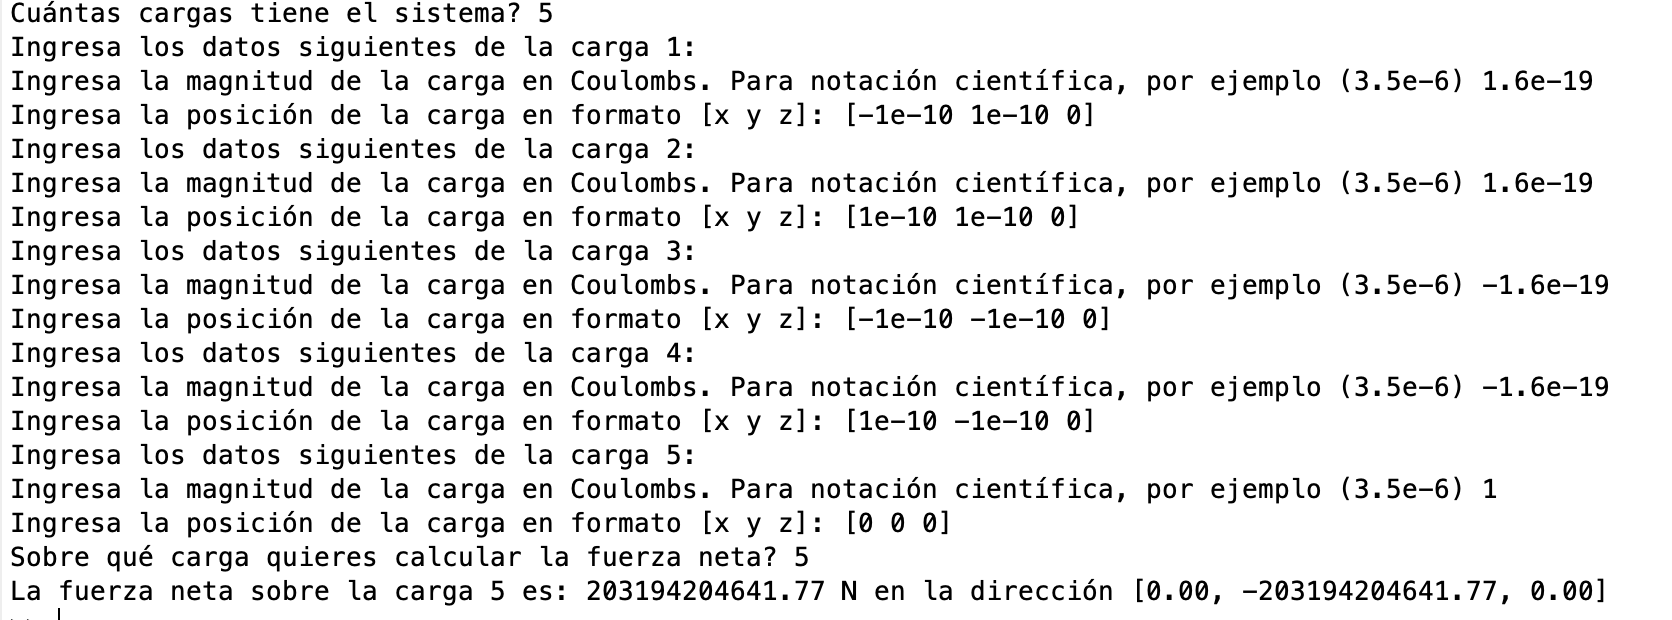
\includegraphics[height = 5cm]{2024-04-27_MatlabEArg1.png}
    \caption{Corrida de código en Matlab}
\end{figure}Al correr el código en Matlab, ingresando adecuadamente las magnitudes y posiciones de todas las cargas, nos resulta que la magnitud de la fuerza eléctrica 
es de $-203194204641.77N$, lo cuál corresponde correctamente y confirma los resultados teóricos obtenidos previamente. \\

Si en cambio quisieramos realizar el análisis con la carga de prueba con magnitud negativa, nos daremos cuenta que obtenemos exactamente el mismo resultado de fuerza eléctrica, 
pero con dirección hacia el eje $y$ positivo. Ésto debido a que se se invierte la magnitud de la fuerza neta porque es negativa en vez de positiva, y por lo tanto 
el vector cambia a la dirección contraria. 
\subsection*{Situación 2}
Otro ingeniero diseña un cañón de electrones el cual proyecta un electrón con una velocidad inicial $v_0=1.60x10^6 m/s$ al interior de una zona con un campo eléctrico uniforme como el que se ilustra en la figura. Lo que sabe sobre el campo eléctrico es que va dirigido hacia abajo y que es igual a cero fuera de las placas. El electrón sale disparado (posición inicial) en el extremo izquierdo y en el punto medio entre las placas (ver figura). 
Pregunta1: Si el electrón pasa rozando la placa superior para luego salir de la zona con campo eléctrico, ¿Cuál es la magnitud de dicho campo eléctrico? 
Pregunta2: ¿Qué pasaría si el camarada Inge dispara ahora un protón bajo las mismas condiciones?\\ 

Solución: 
En éste problema, tenemos una situación en donde una partícula entra a un campo eléctrico que se dirige en dirección $Y$ negativa. Para encontrar qué sucede 
con el campo eléctrico en el punto en el que el electrón sale rozando, hay que hacer un análisis de fuerzas y tratar de encontrar una fórmula para el campo eléctrico. Podemos observar que 
como la partícula se mueve en dirección X positiva, y no existe ninguna fuerza que se oponga al movimiento en X, su velocidad en X es constante, y por lo tanto $V_x = V_0 = 1.60x10^-6m/s$. \\

Como la posición es la integral de velocidad, integramos la fórmula anterior para obtener la posición en X respecto al tiempo, es decir: $x_x(t) = \int V_x(t)dt = 1.60x10^6t$. De aquí, sabiendo que 
la posición final es $0.02m$, podemos sustituir y despejar en la fórmula de posición en $x$ para obtener el tiempo. Entonces: $0.02m = 1.60x10^6 t$, y por lo tanto $t = 1.25x10^-8s$. Ahora, una vez que tenemos el tiempo, es conveniente analizar las fuerzas 
en Y, para obtener una fórmula de posición que nos permita saber la mangitud del campo eléctrico en cualquier punto de la trayectoria. \\ 

En Y, solo existe la fuerza de gravedad y la fuerza eléctrica, por lo tanto $F_y = -mg(q\vec{E})$. Sabemos que, de acuerdo a Netwon, $F = ma$, entonces la suma de fuerzas en Y debe ser igual a $ma_y$, es decir, $ma_y = -mg(q\vec{E})$. De aquí, podemos obtener 
una fórmula para la aceleración en $y$ despejando ésta variable, lo cuál resulta $a_y = -g + \frac{q\vec{E}}{m}$. Sabiendo que la aceleración es la segunda derivada de la posición, integramos dos veces 
para obtener una fórmula para posición en Y, lo cuál resulta $x_y(t) = -\frac{gt^2}{2} + \frac{qt^2}{2m}E$. Las constantes de integración se anulan ya que tanto la posición inicial en Y como la 
velocidad inicial en Y son 0, y por lo tanto las constantes no tienen efecto en el resultado de la integral. Después, como sabemos que cuando la partícula sale del campo eléctrico su posición es de 
(0, 0) y cuando roza la placa superior su posición en $y$ es de 0.005m, usamos esos datos junto con la masa del electrón $m = 9.1x10^-31 kg$, la carga del electrón $q = -1.6x10^-19 C$, y el tiempo obtenido 
previamente $t = 1.25x10^-8s$, el valor de la gravedad $g = 9.81$ y sustituimos esos datos en la fórmula obtenida de posición en Y, lo cuál nos permite despejar el campo eléctrico: 
\begin{align}
0.01 &= -\frac{9.81(1.25x10^-8)^2}{2}+\frac{-1.6x10^-19(1.25x10^-8)^2}{2(9.1x10^-31)}E\\
\intertext{Y despejando para el campo eléctrico E}
E &= -364 \frac{V}{M}
\end{align}Eso quiere decir que magnitud del campo eléctrico cuando el electrón roza la placa superior es de $E = -364 \frac{V}{m}$. Ésto es congruente ya que 
como se indica en el problema, el campo eléctrico es negativo debido a que apunta hacia abajo, es decir, el extremo positivo es la placa superior, y el extremo negativo es la placa inferior, y por lo tanto 
el campo va siempre del lado positivo al negativo. \\ 

Ahora, si el ingeniero decidiera disparar un protón bajo las mismas condiciones, lo que pasaría es que tendría exactamente el efecto contrario, es decir, la partícula en vez de dirigirse hacia la parte superior, 
se dirigiría hacia la parte inferior ya que el protón tiene carga positiva, y como las cargas opuestas se atraen, eso significa que la carga positiva se verá atraida hacia la placa negativa, que se encuentra en la parte 
inferior del sistema. A nivel de campo eléctrico, puede que sea diferente debido a que la masa del protón es diferente a la del electrón, y como el campo eléctrico se multiplica por la masa en las fórmulas anteriores, 
puede que la magnitud sea diferente. 

\subsection*{Situación 3}
En el circuito 1, para encontrar las corrientes eléctricas, se hace un análisis con la técnica de nodos, que consiste en 
definir puntos en el circuito donde se interconectan 2 o más elementos del circuito, y basandose en las Leyes de Kirchoff, que dicen que la corriente que entra a 
un nodo es la misma que la que sale, es decir, la suma de corrientes es igual a cero. Además, usamos la Ley de Ohm, que nos dice que el voltaje es igual al producto de la 
resistencia por la corriente, es decir, $V = RI$. Despejando para la coriente, $I = V/R$, donde $V$ se refiere a la diferencia de potencial entre dos nodos. 
Por lo tanto, primero definimos los nodos, como se muestra en la siguiente imagen: 
\begin{figure}[H]
    \centering
    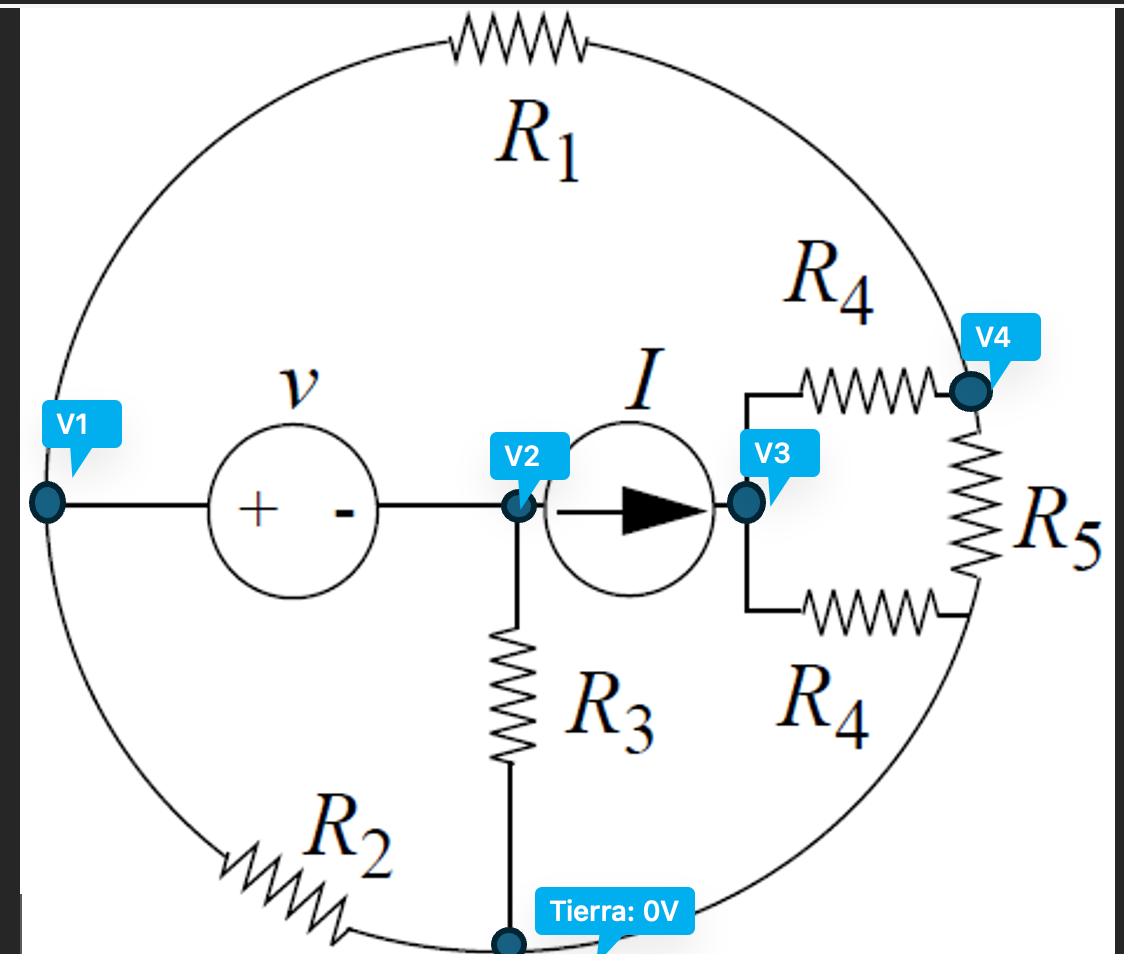
\includegraphics[height = 4cm]{Diagrama1.png}
    \caption{Diagrama de nodos para el circuito 1}
\end{figure}
Por lo tanto, se tiene que hacer un sistema de ecuaciones de 4X4, ya que quedan 4 nodos o corrientes por resolver. Además, contamos con un supernodo entre 1 y 2, 
que al estar conectados por la pila, podemos combinar sus ecuaciones nodales y además establecer la relación que existe entre ambos por medio de la pila. Entonces, se hacen las ecuaciones nodales 
tomando en cuenta lo anterior. Una vez obtenidas las ecuaciones nodales, se pueden reescribir, de manera que se aislan las variables y nos permite crear un sistema de ecuaciones de tipo $A\vec{x} = \vec{b}$, donde 
$A$ corresponde a la matriz de coeficientes, $\vec{x}$ corresponde a la matriz de incógnitas, y $\vec{b}$ a la matriz del lado derecho con los resultados. Una vez hecho ésto, se puede ingresar ésta matriz 
a Matlab y obtener la solución del circuito. A continuación se muestran los procedimientos: 
\begin{figure}[H]
    \centering
    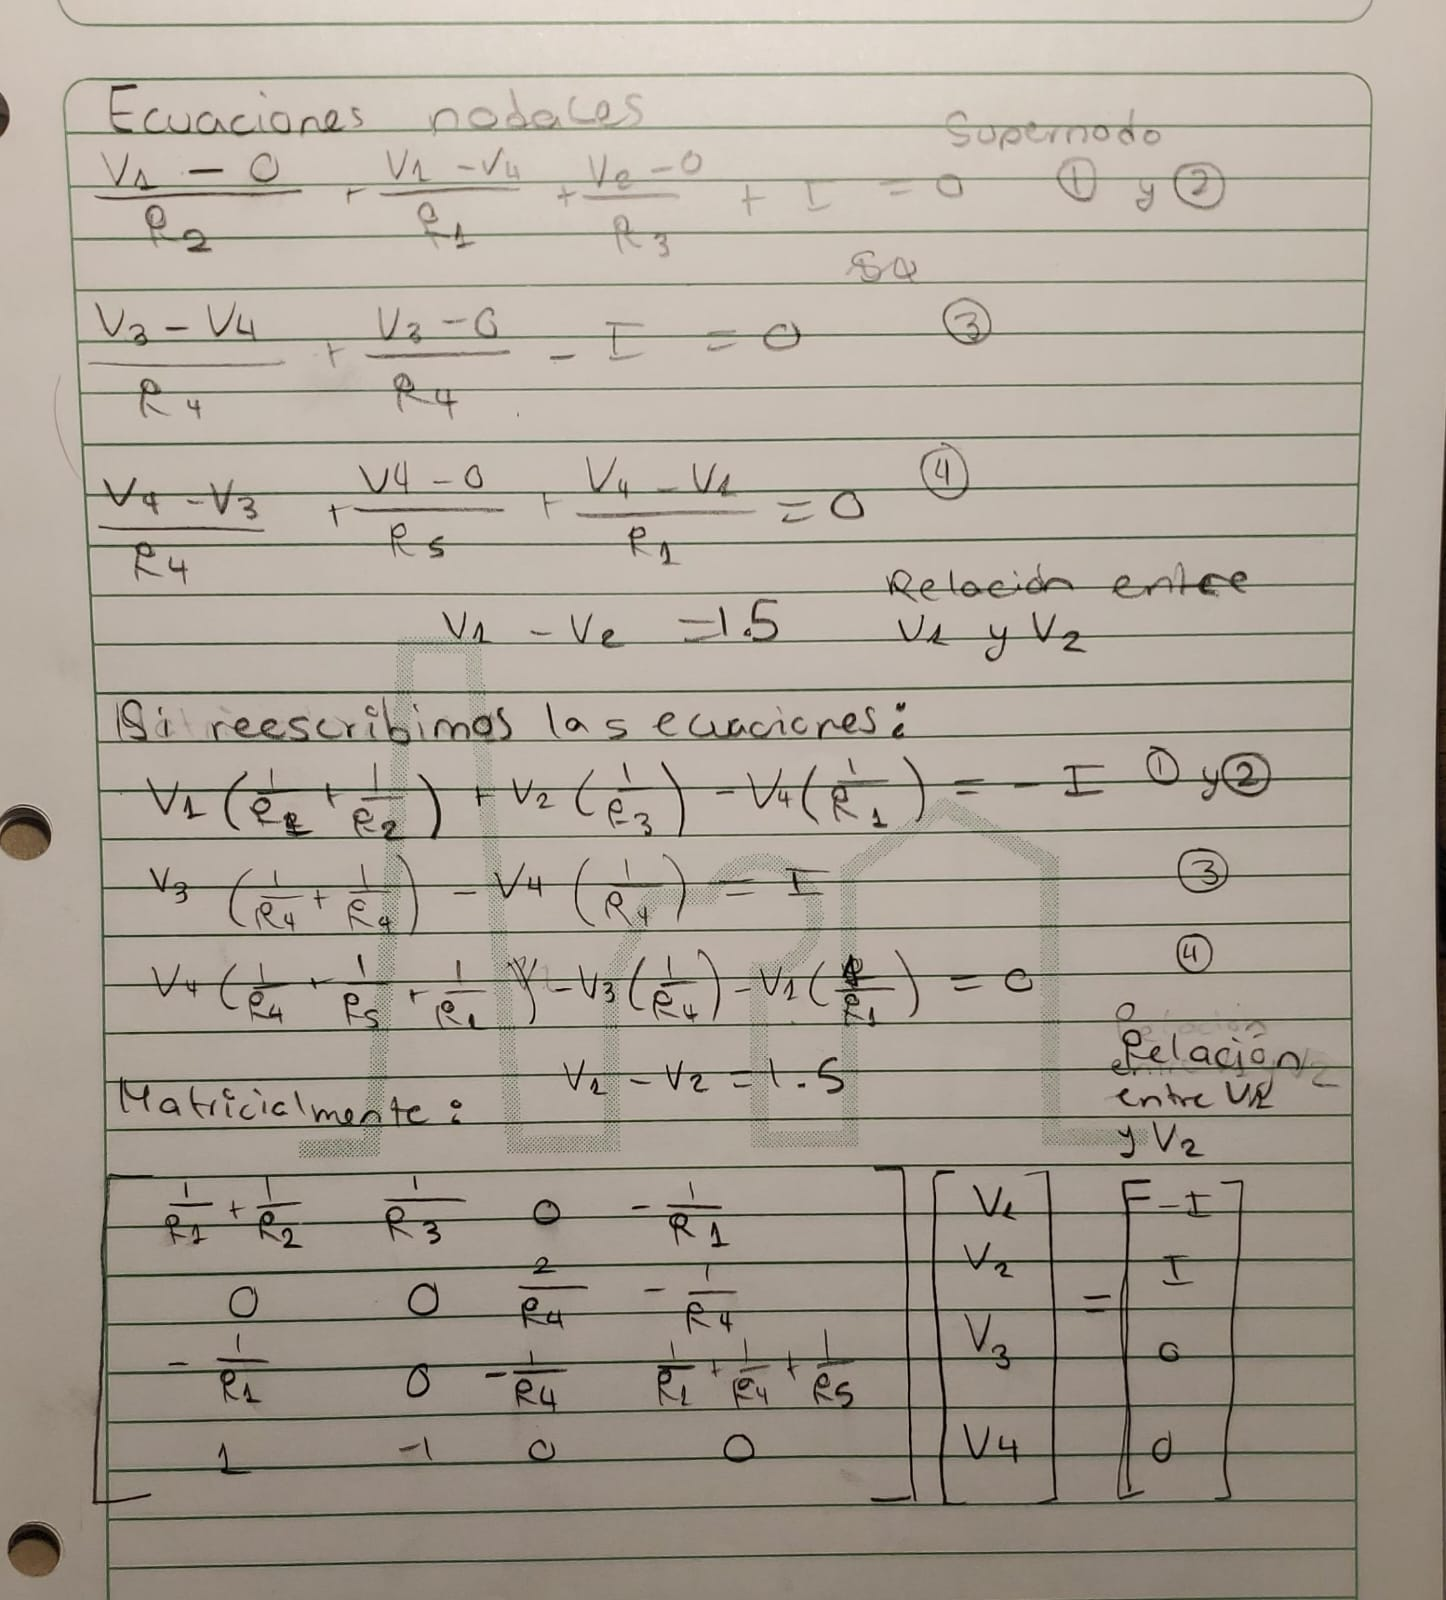
\includegraphics[height = 12cm]{Operaciones_1.jpeg}
    \caption{Hoja de operaciones para el circuito 1}
\end{figure}
Así, ingresando las matrices en Matlab, resulta que $V_1 = 0.7656V$, $V_2 = -0.7344$, $V_3 = 0.0482V$ y $V_4 = 0.0958$. Después, usando igualmente la Ley de Ohm, calculamos las corrientes de cada resistencia, y vemos 
que no hay ninguna corriente en serie, ya que no hay dos corrientes de la misma magnitud: 
\begin{figure}[H]
    \centering
    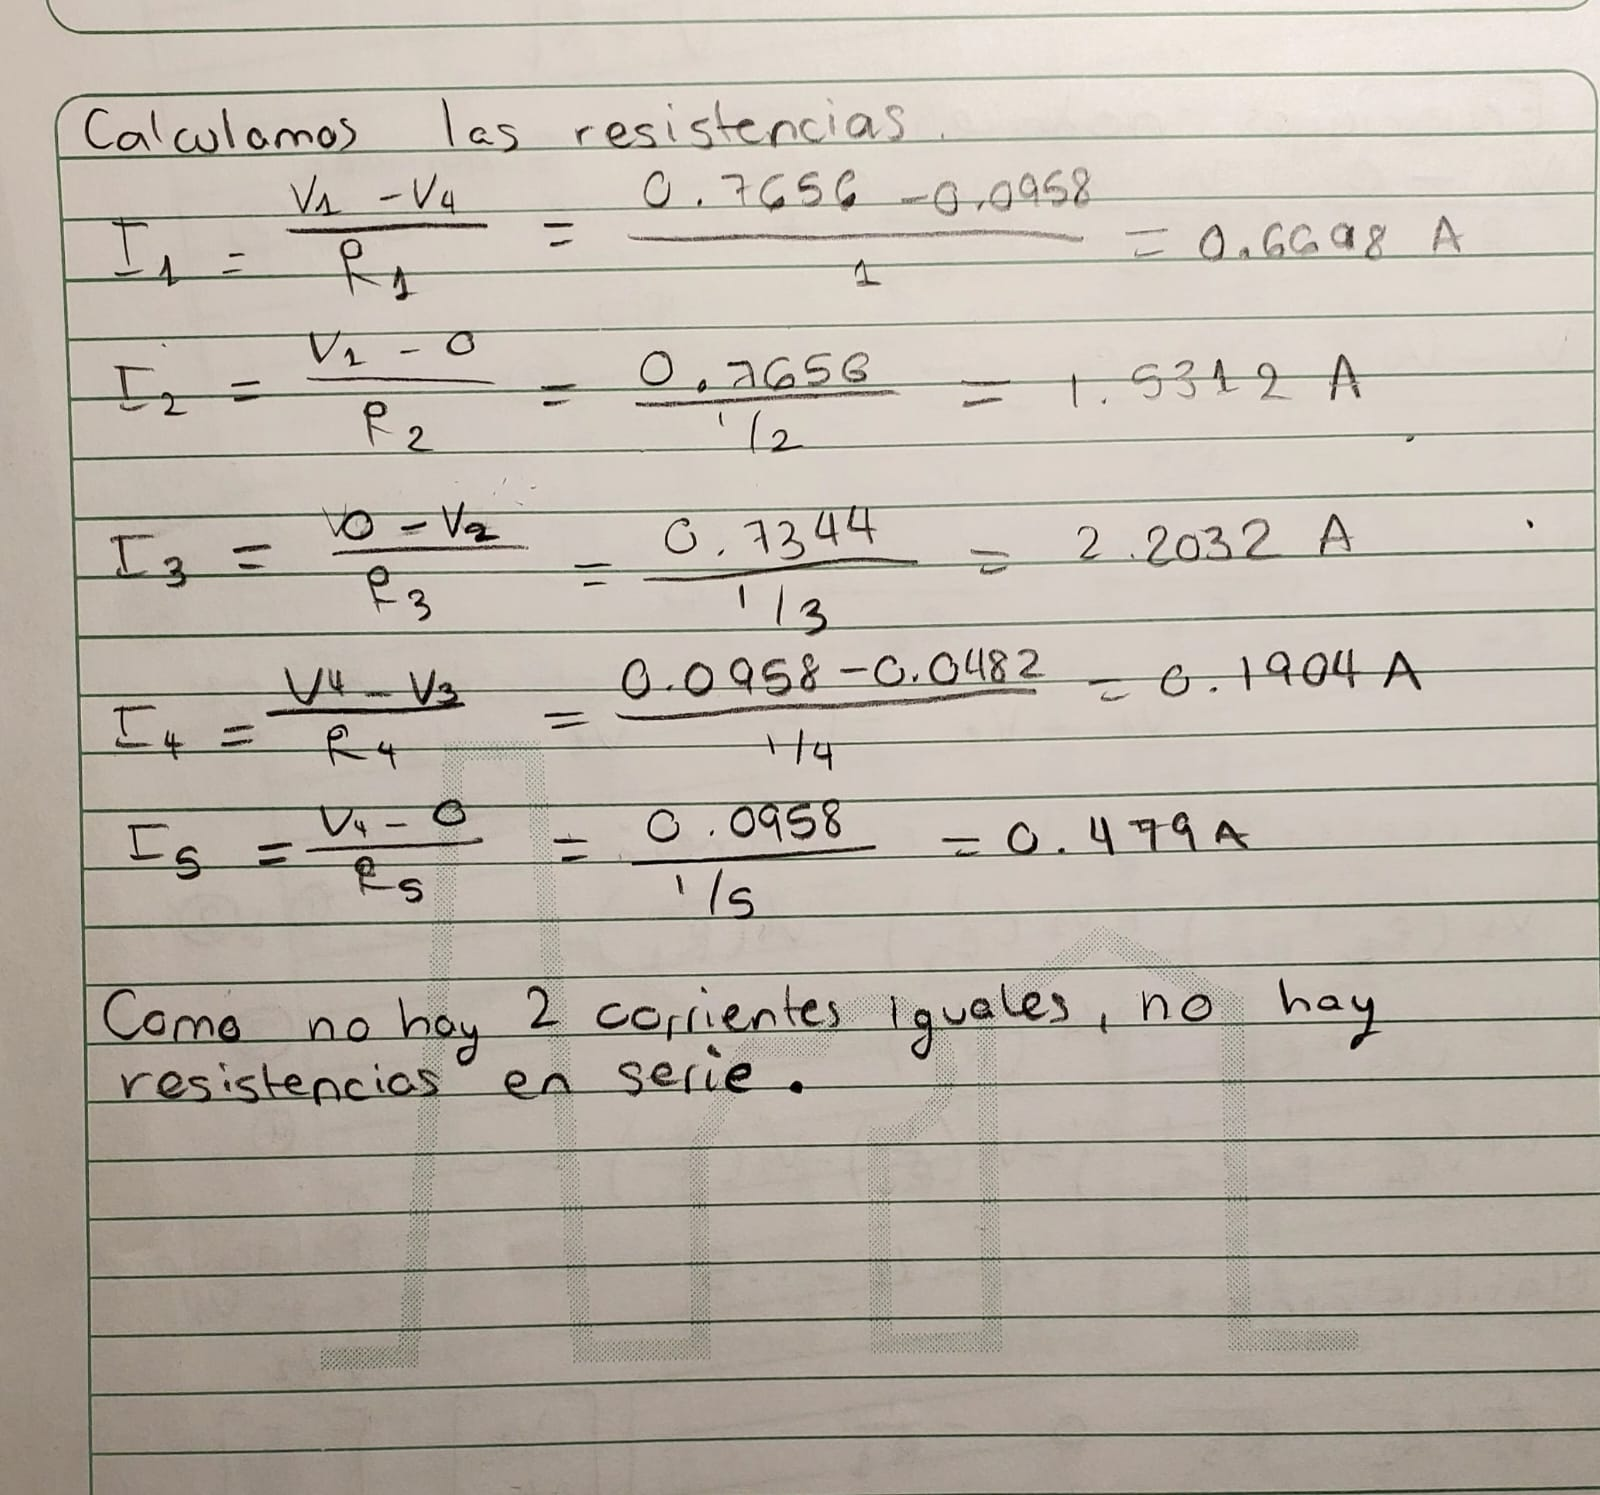
\includegraphics[height = 10cm]{Corrientes 1.jpeg}
    \caption{Cálculo de corrientes para el circuito 1}
\end{figure}
\textbf{Circuito 2: }
Análogamente al circuito 1, en éste circuito igualemnte se usa la técnica de análisis de nodos para encontrar los voltajes. Éste es un circuito muy práctico ya que 
debido a su arreglo en forma de diamante, nos permite seleccionar la tierra, y por lo tanto resolver un nodo, pasando de 5 nodos a 3 nodos sin resolver. A continuación se muestran las ecuaciones nodales, la manera 
en la que se reescribieron para acomodarlas de manera que se convierta en un sistema de ecuaciones, y su representación matricial: 
\begin{figure}[H]
    \centering
    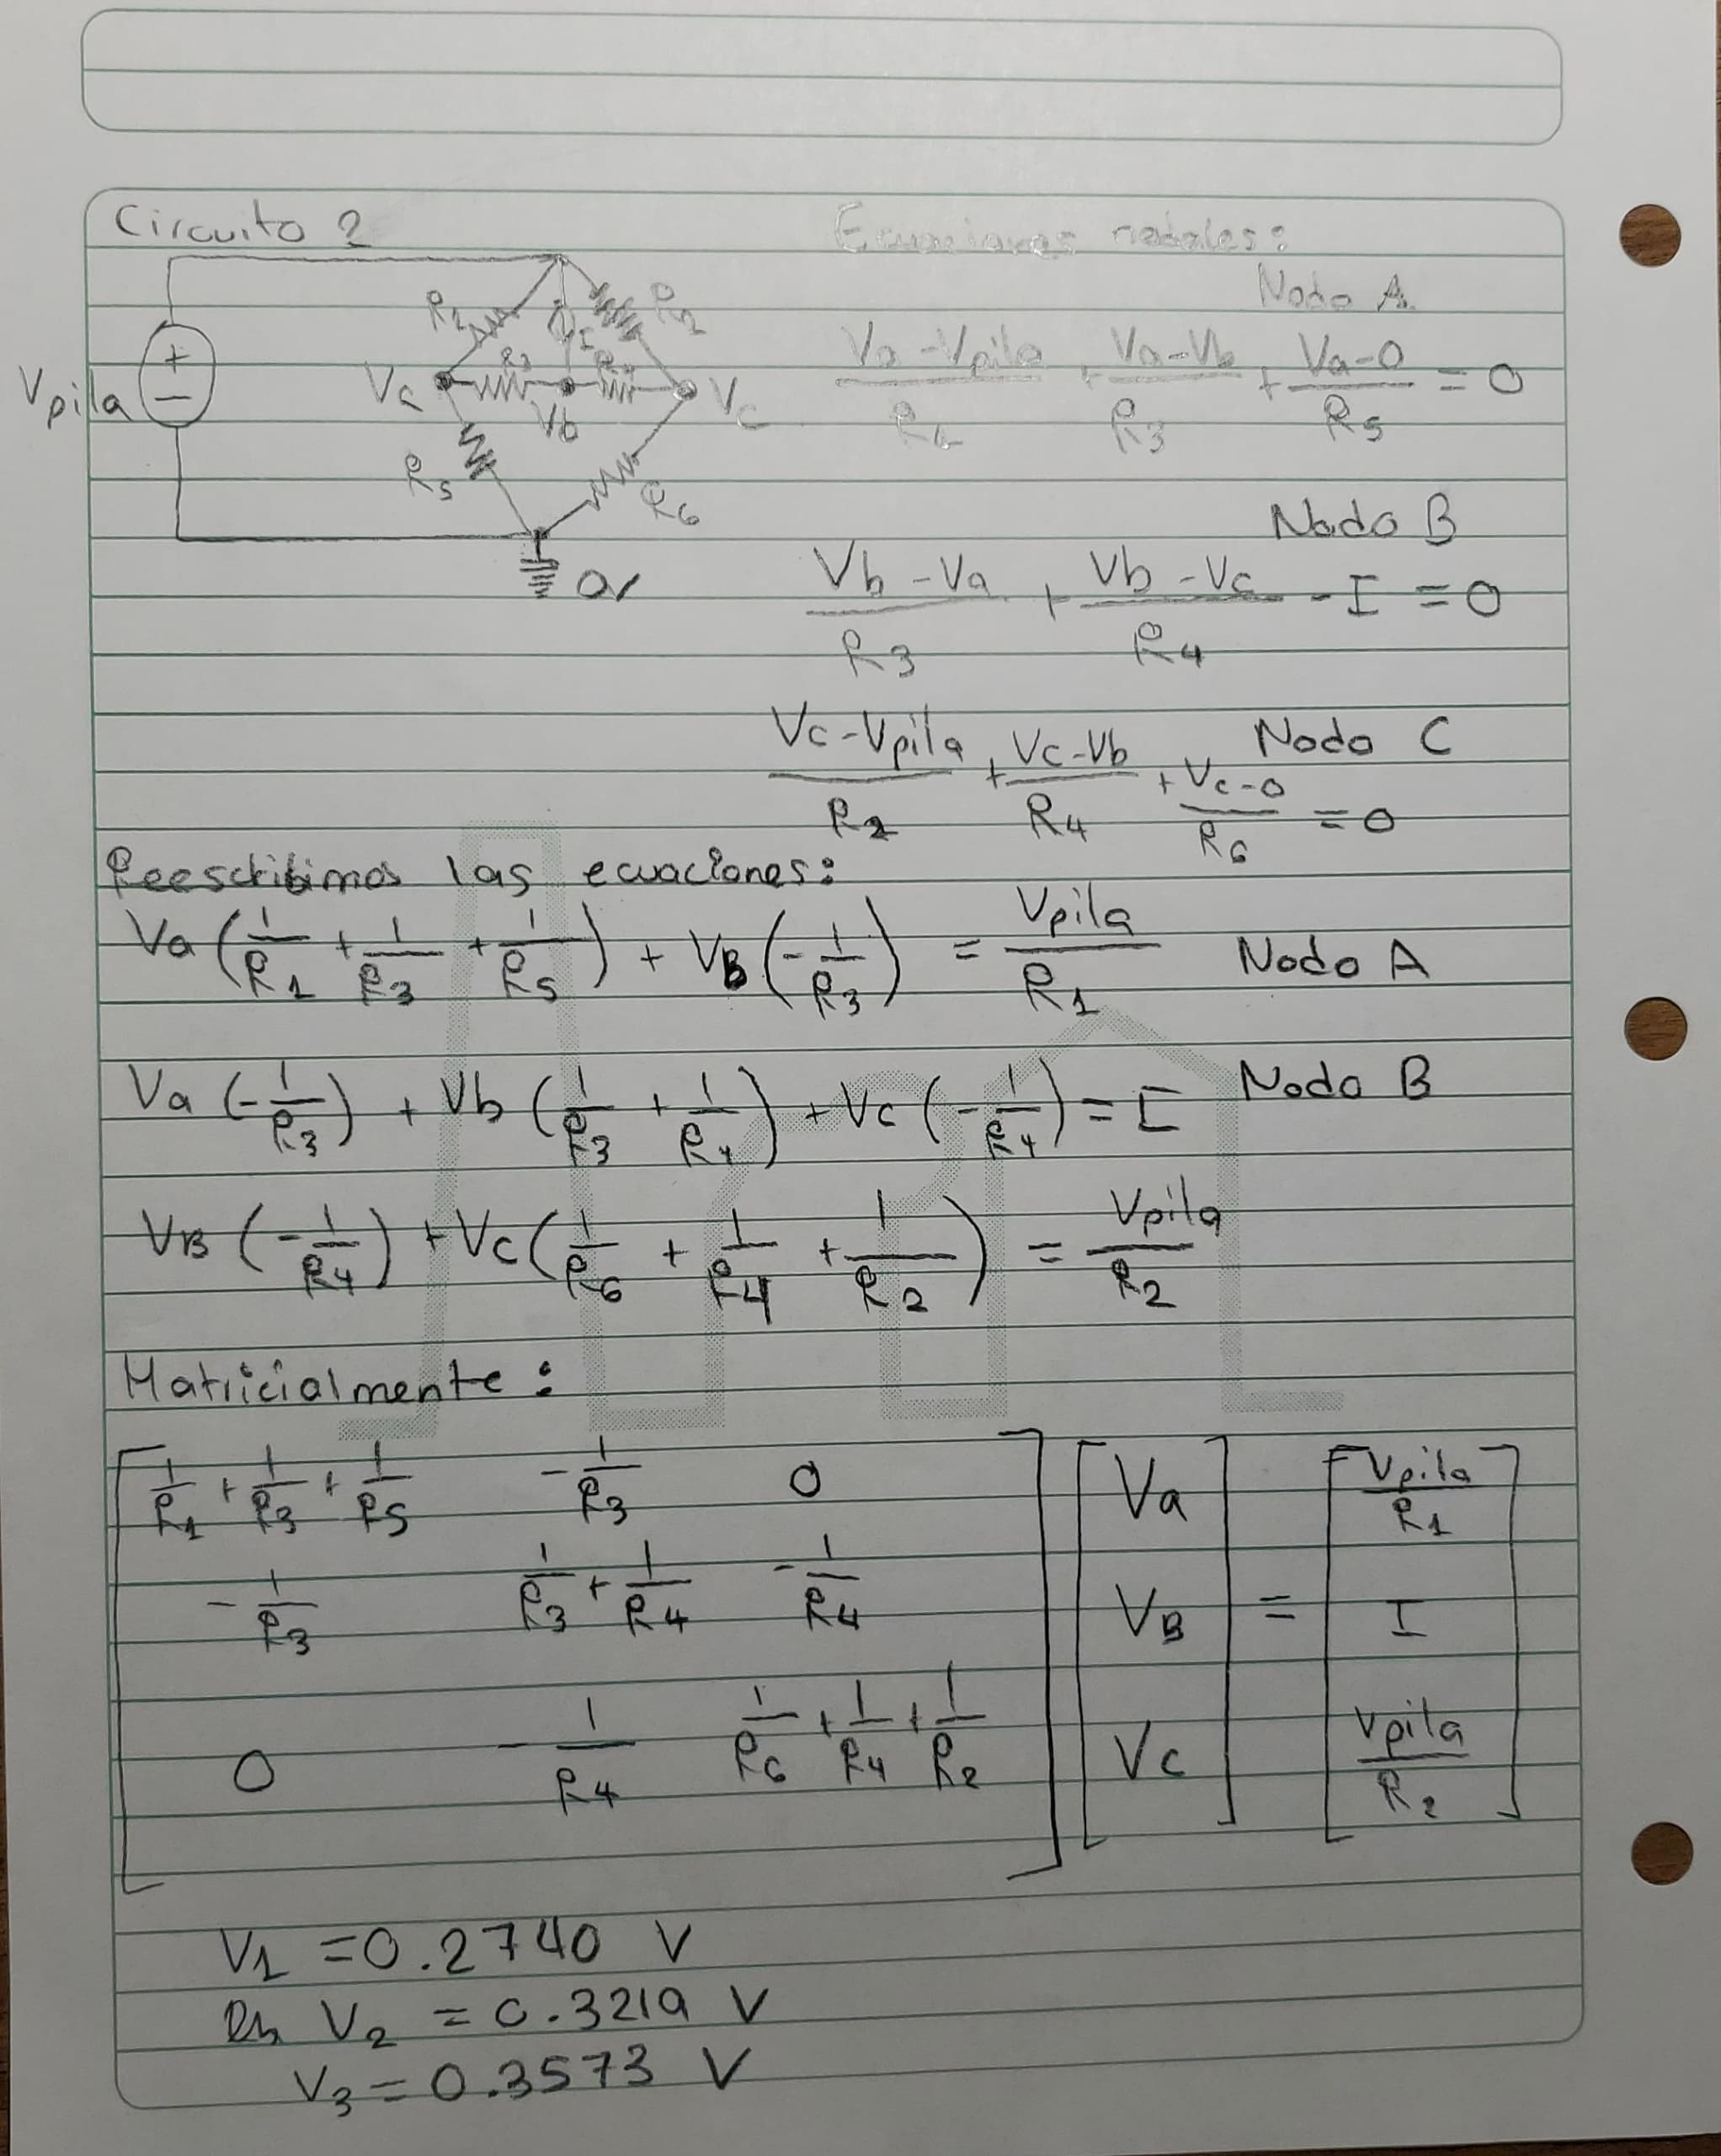
\includegraphics[height = 12cm]{corrientes 2.jpeg}
    \caption{Cálculo de voltajes para el circuito 2}
\end{figure}Si ingresamos el sistema de ecuaciones a Matlab, podemos obtener la solución al sistema de ecuaciones que nos dará la solución a los voltajes en cada uno de los nodos. Así, resulta $V_a = 0.2740 V$, 
$V_b = 0.3219 V$, y $V_c = 0.3573V$. Éstos voltajes son correctos ya que son consistentes en magnitud con lo esperado, es decir, su magnitud es la adecuada para las dimensiones y magnitudes 
del circuito. Después, podemos calcular las corrientes: 
\begin{figure}[H]
    \centering
    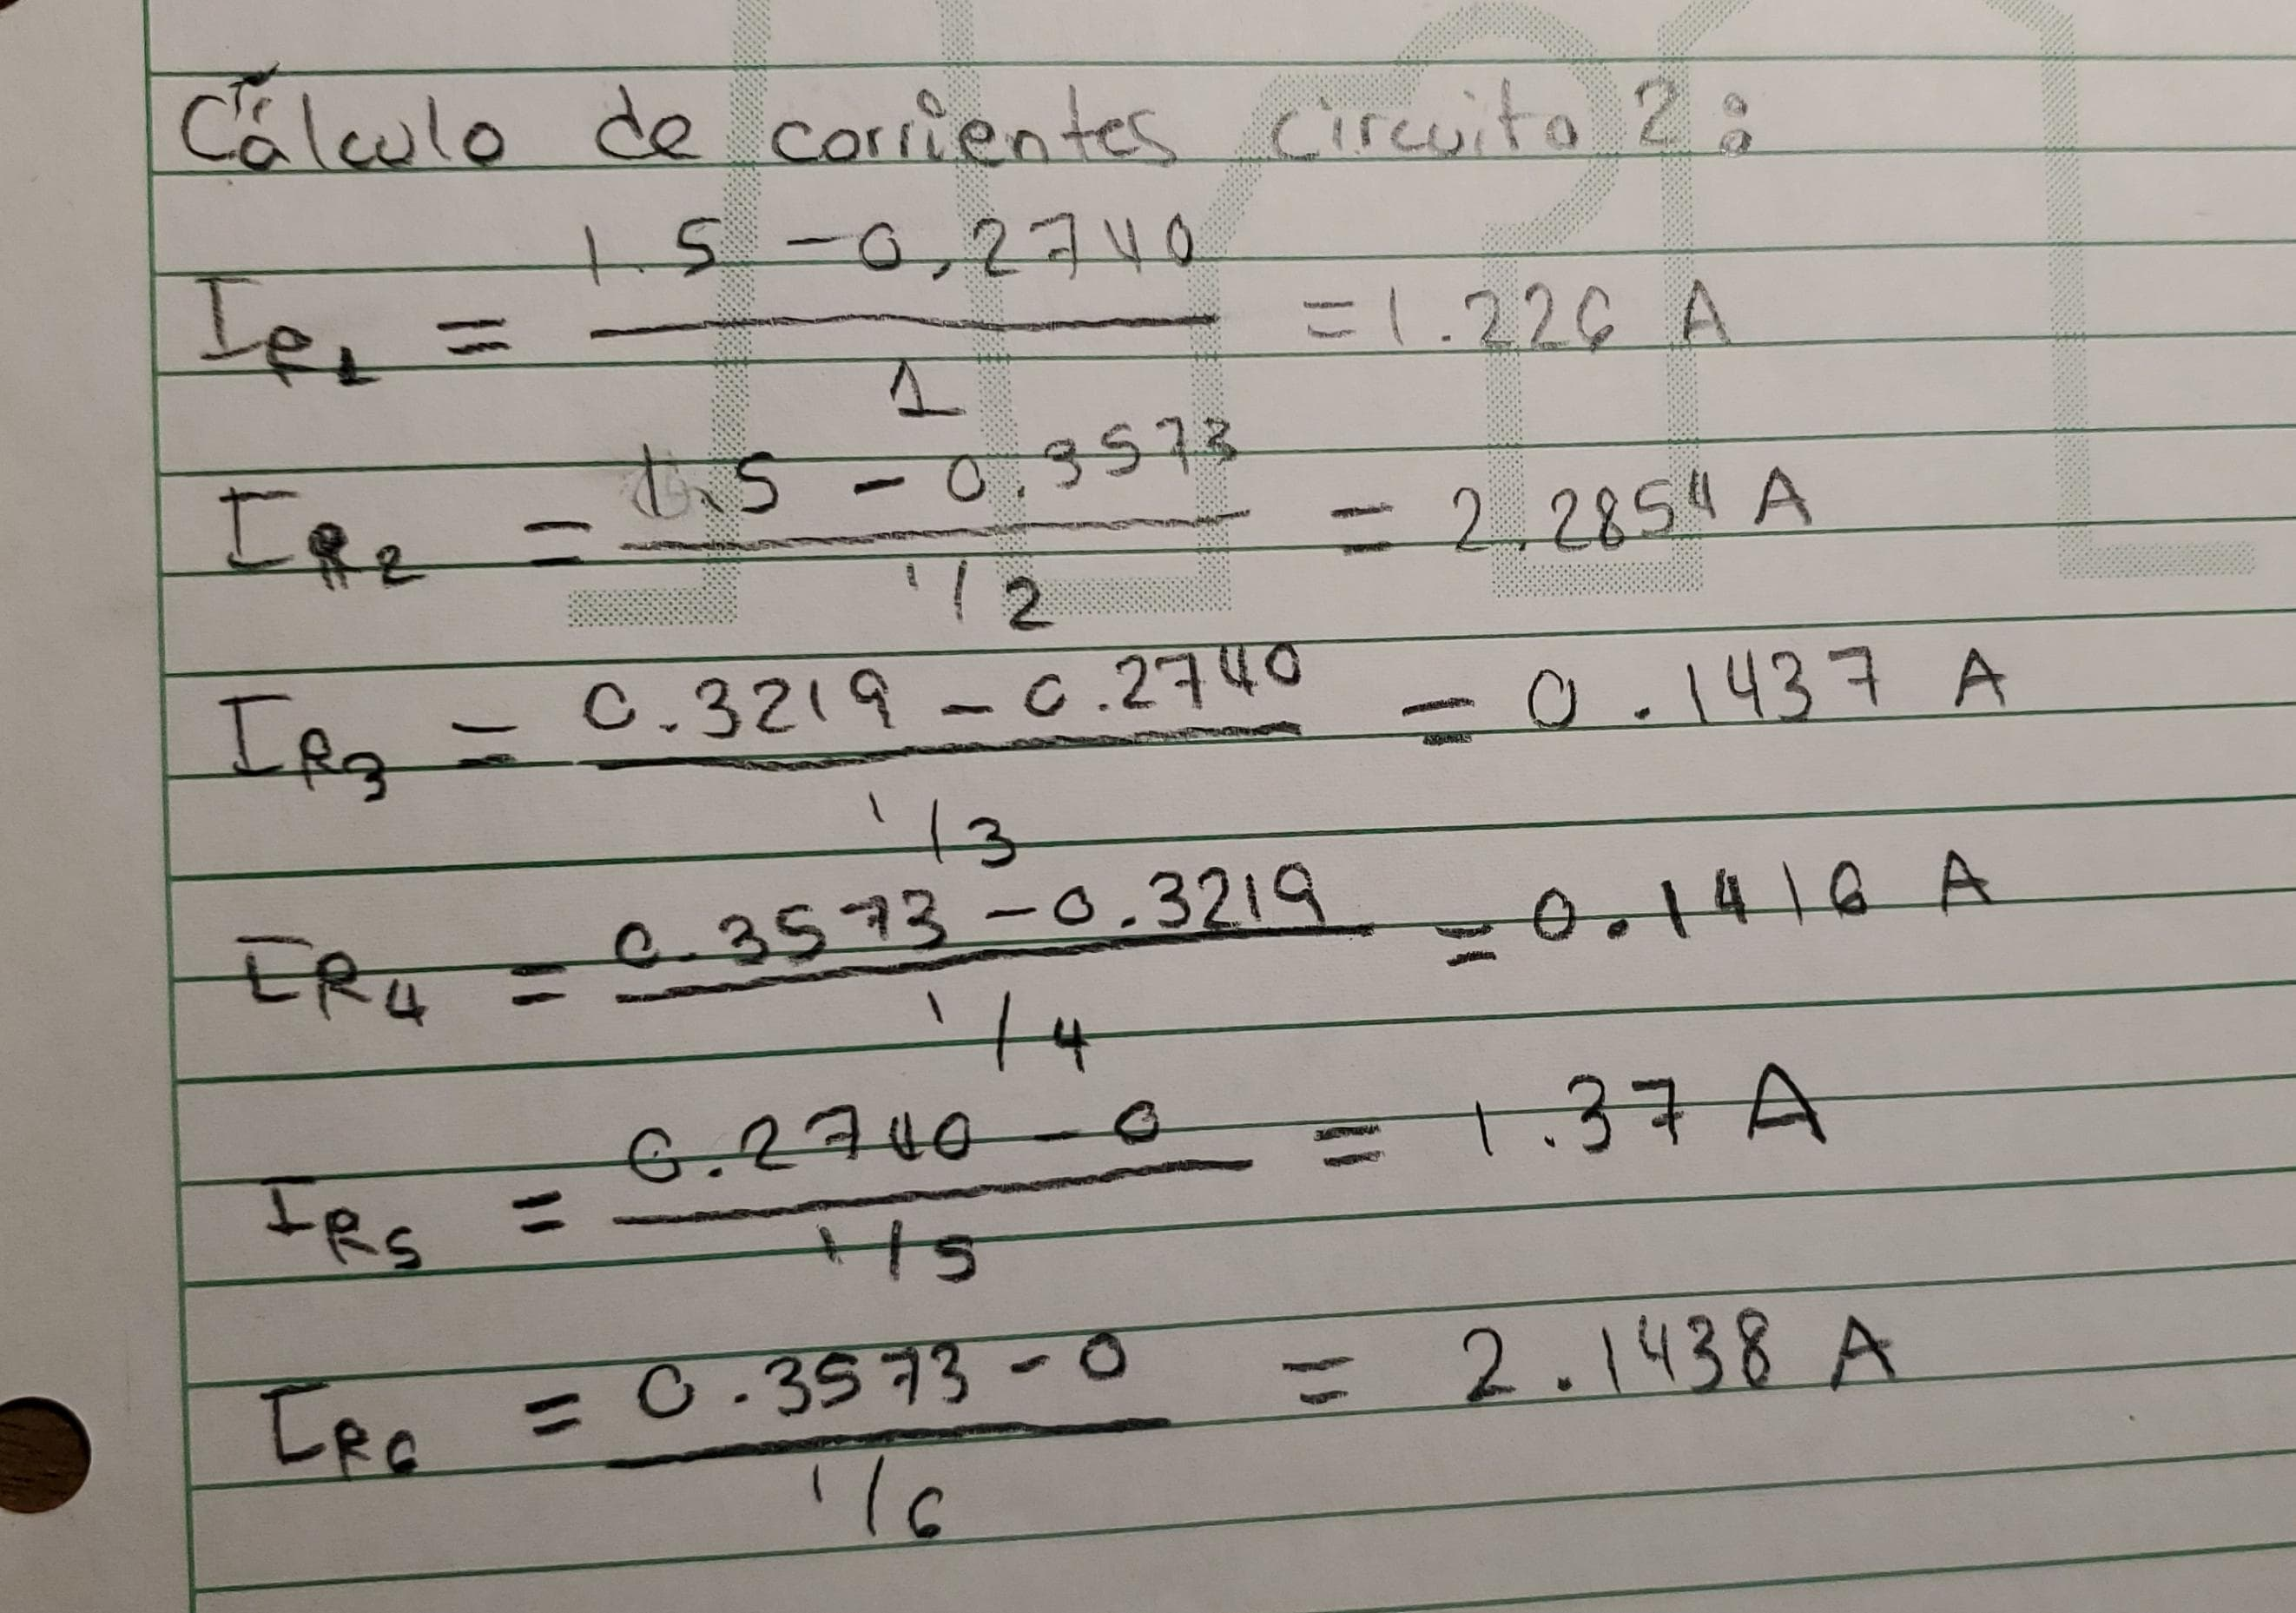
\includegraphics[height = 8cm]{corrientes 3.jpeg}
    \caption{Cálculo de corrientes de circuito 2}
\end{figure}Igual que en el circuito anterior, podemos ver que no existen resistencias en serie, ya que no hay dos resistencias con el mismo valor. 

\end{document}